%% Support sites:
%% http://www.michaelshell.org/tex/ieeetran/
%% http://www.ctan.org/tex-archive/macros/latex/contrib/IEEEtran/
%% and
%% http://www.ieee.org/

% Also note that the "draftcls" or "draftclsnofoot", not "draft", option
% should be used if it is desired that the figures are to be displayed in
% draft mode.
%
\documentclass[conference]{IEEEtran}
% Add the compsoc option for Computer Society conferences.

\usepackage{flushend}
%\usepackage{ifpdf}
\usepackage{cite}
\usepackage{pgfplots}
\usepackage{microtype}


%\usepackage{booktabs}

% *** GRAPHICS RELATED PACKAGES ***
%
\ifCLASSINFOpdf
  % \usepackage[pdftex]{graphicx}
  % declare the path(s) where your graphic files are
  % \graphicspath{{../pdf/}{../jpeg/}}
  % and their extensions so you won't have to specify these with
  % every instance of \includegraphics
  % \DeclareGraphicsExtensions{.pdf,.jpeg,.png}
\else
  % or other class option (dvipsone, dvipdf, if not using dvips). graphicx
  % will default to the driver specified in the system graphics.cfg if no
  % driver is specified.
  % \usepackage[dvips]{graphicx}
  % declare the path(s) where your graphic files are
  % \graphicspath{{../eps/}}
  % and their extensions so you won't have to specify these with
  % every instance of \includegraphics
  % \DeclareGraphicsExtensions{.eps}
\fi
% graphicx was written by David Carlisle and Sebastian Rahtz. It is
% required if you want graphics, photos, etc. graphicx.sty is already
% installed on most LaTeX systems. The latest version and documentation can
% be obtained at:
% http://www.ctan.org/tex-archive/macros/latex/required/graphics/
% Another good source of documentation is "Using Imported Graphics in
% LaTeX2e" by Keith Reckdahl which can be found as epslatex.ps or
% epslatex.pdf at: http://www.ctan.org/tex-archive/info/
%
% latex, and pdflatex in dvi mode, support graphics in encapsulated
% postscript (.eps) format. pdflatex in pdf mode supports graphics
% in .pdf, .jpeg, .png and .mps (metapost) formats. Users should ensure
% that all non-photo figures use a vector format (.eps, .pdf, .mps) and
% not a bitmapped formats (.jpeg, .png). IEEE frowns on bitmapped formats
% which can result in "jaggedy"/blurry rendering of lines and letters as
% well as large increases in file sizes.
%
% You can find documentation about the pdfTeX application at:
% http://www.tug.org/applications/pdftex

\usepackage[cmex10]{amsmath}
%\usepackage{amssymb}

% *** SPECIALIZED LIST PACKAGES ***
%
%\usepackage{algorithmic}
% algorithmic.sty was written by Peter Williams and Rogerio Brito.
% This package provides an algorithmic environment fo describing algorithms.
% You can use the algorithmic environment in-text or within a figure
% environment to provide for a floating algorithm. Do NOT use the algorithm
% floating environment provided by algorithm.sty (by the same authors) or
% algorithm2e.sty (by Christophe Fiorio) as IEEE does not use dedicated
% algorithm float types and packages that provide these will not provide
% correct IEEE style captions. The latest version and documentation of
% algorithmic.sty can be obtained at:
% http://www.ctan.org/tex-archive/macros/latex/contrib/algorithms/
% There is also a support site at:
% http://algorithms.berlios.de/index.html
% Also of interest may be the (relatively newer and more customizable)
% algorithmicx.sty package by Szasz Janos:
% http://www.ctan.org/tex-archive/macros/latex/contrib/algorithmicx/

\usepackage{listings}


\usepackage{array}
\usepackage{mdwmath}
\usepackage{mdwtab}

\usepackage{eqparbox}
%\usepackage[tight,footnotesize]{subfigure}
%\usepackage[caption=false]{caption}
\usepackage[caption=false, font=footnotesize]{subfig}
% subfig.sty, also written by Steven Douglas Cochran, is the modern
% replacement for subfigure.sty. However, subfig.sty requires and
% automatically loads Axel Sommerfeldt's caption.sty which will override
% IEEEtran.cls handling of captions and this will result in nonIEEE style
% figure/table captions. To prevent this problem, be sure and preload
% caption.sty with its "caption=false" package option. This is will preserve
% IEEEtran.cls handing of captions. Version 1.3 (2005/06/28) and later
% (recommended due to many improvements over 1.2) of subfig.sty supports
% the caption=false option directly:
%\usepackage[caption=false,font=footnotesize]{subfig}
%
% The latest version and documentation can be obtained at:
% http://www.ctan.org/tex-archive/macros/latex/contrib/subfig/
% The latest version and documentation of caption.sty can be obtained at:
% http://www.ctan.org/tex-archive/macros/latex/contrib/caption/




% *** FLOAT PACKAGES ***
%
%\usepackage{fixltx2e}
% fixltx2e, the successor to the earlier fix2col.sty, was written by
% Frank Mittelbach and David Carlisle. This package corrects a few problems
% in the LaTeX2e kernel, the most notable of which is that in current
% LaTeX2e releases, the ordering of single and double column floats is not
% guaranteed to be preserved. Thus, an unpatched LaTeX2e can allow a
% single column figure to be placed prior to an earlier double column
% figure. The latest version and documentation can be found at:
% http://www.ctan.org/tex-archive/macros/latex/base/



%\usepackage{stfloats}
% stfloats.sty was written by Sigitas Tolusis. This package gives LaTeX2e
% the ability to do double column floats at the bottom of the page as well
% as the top. (e.g., "\begin{figure*}[!b]" is not normally possible in
% LaTeX2e). It also provides a command:
%\fnbelowfloat
% to enable the placement of footnotes below bottom floats (the standard
% LaTeX2e kernel puts them above bottom floats). This is an invasive package
% which rewrites many portions of the LaTeX2e float routines. It may not work
% with other packages that modify the LaTeX2e float routines. The latest
% version and documentation can be obtained at:
% http://www.ctan.org/tex-archive/macros/latex/contrib/sttools/
% Documentation is contained in the stfloats.sty comments as well as in the
% presfull.pdf file. Do not use the stfloats baselinefloat ability as IEEE
% does not allow \baselineskip to stretch. Authors submitting work to the
% IEEE should note that IEEE rarely uses double column equations and
% that authors should try to avoid such use. Do not be tempted to use the
% cuted.sty or midfloat.sty packages (also by Sigitas Tolusis) as IEEE does
% not format its papers in such ways.


\usepackage{url}
\usepackage{epstopdf}



% *** Do not adjust lengths that control margins, column widths, etc. ***
% *** Do not use packages that alter fonts (such as pslatex).         ***
% There should be no need to do such things with IEEEtran.cls V1.6 and later.
% (Unless specifically asked to do so by the journal or conference you plan
% to submit to, of course. )


% correct bad hyphenation here
\hyphenation{op-tical net-works semi-conduc-tor}

\usepackage[normalem]{ulem}
\usepackage{tikz}
\usepackage{xcolor}
\usepackage{lipsum}
\usepackage{verbatim}
\usepackage{multirow}
\usepackage{multicol}
\usetikzlibrary{shapes,arrows,fit}

\tikzstyle{decision} = [diamond, draw, fill=blue!20, text width=4.5em,
text badly centered, node distance=3cm, inner sep=0pt]

\tikzstyle{block} = [rectangle, draw, fill=blue!20, text width=5em,
text centered, rounded corners, minimum height=4em]

\tikzstyle{line} = [draw, -latex'] \tikzstyle{cloud} = [draw,
ellipse,fill=red!20, node distance=3cm, minimum height=2em]

\newcommand{\XXX}[1]{{\bf \color{red} XXX: #1}}
\newcommand{\TODO}[0]{{\bf \color{red} TODO\ }}
\newcommand{\MAXC}[0]{FAST}
\newcommand\reduline{\bgroup\markoverwith
  {\textcolor{red}{\rule[-0.5ex]{2pt}{0.4pt}}}\ULon}
\newcommand{\FIC}[1]{\reduline{#1}}
\newcommand{\blt}{\raise .2ex\hbox{\tiny$\bullet$ }}

%\usepackage[margin=1cm]{caption}

\newcounter{nodemarkers}
\newcommand\marktext[1]{%
    \tikz[overlay,remember picture]
        \node (marker-\arabic{nodemarkers}-a) at (0,1.5ex) {};%
    #1%
    \tikz[overlay,remember picture]
        \node (marker-\arabic{nodemarkers}-b) at (0,0){};%
    \tikz[overlay,remember picture,inner sep=2pt]
        \node[draw,dotted,rectangle,fit=(marker-\arabic{nodemarkers}-a.center) (marker-\arabic{nodemarkers}-b.center)] {};%
    \stepcounter{nodemarkers}%
}

\begin{document}

\captionsetup{width=2cm}
\lstset{escapeinside={(*@}{@*)}}
\lstdefinestyle{lara}{ language=C++, breaklines=true, % frame=tb,
  xleftmargin=2em, numbers=left, captionpos=b,
  morekeywords={aspectdef, var, apply, select, condition, begin, end, input}}

\lstdefinestyle{MaxC}{language=C++, breaklines=true, %frame=tb,
  xleftmargin=2em, numbers=left,
  captionpos=b,basicstyle=\ttfamily\footnotesize,
  morekeywords={s_int32, int32, float8_24, sin_float8_24,
    sout_float8_24, float8_24, s_int, s_float8_24, s_bool},
    deletekeywords={static}}

\title{Aspect Driven Compilation for \\ Dataflow Designs}

\author{
  \IEEEauthorblockN{
    \emph{Paul Grigora\c{s}},
    \emph{Xinyu Niu},
    \emph{Jose G. F. Coutinho} \and
    \emph{Wayne Luk} \vspace {0.3cm}
  }
  \IEEEauthorblockA{
    Department of Computing, Imperial College London, 180 Queen's Gate, London SW7 2AZ, UK
  }
  \vspace{0.15cm}
  \IEEEauthorblockA{
   Email: \{paul.grigoras09, niu.xinyu10, gabriel.figueiredo, w.luk\}@imperial.ac.uk
  }
}

\maketitle

\begin{abstract}
  We propose a novel design flow for generating dataflow designs based
  on Aspect-oriented programming. We propose to decouple design
  optimisation from design specification by encapsulating
  optimisations in separate aspect descriptions. To support this
  approach we introduce a novel dataflow language that facilitates
  integration with existing aspect weaving tools and simplifies design
  development.
\end{abstract}


\IEEEpeerreviewmaketitle

\section{Introduction}
 \begin{frame}


      \frametitle{Introduction}
      %------------------------------------------------------------ 1
      \only<1>{
        \framesubtitle{Overview}

      }

      \only<2>{
        \framesubtitle{Motivation}
      }

      \only<3>{
        \framesubtitle{Challenges}
      }

      \only<4>{
        \framesubtitle{Contributions
}
      }
  \end{frame}

\chapter{Design Flow}
\label{sec:design-flow}

In this chapter we introduce a novel design flow for creating
high-performance dataflow designs starting from C/C++ applications. We
explain the motivation and requirements for the proposed approach and
provide an overview of the three main components: \emph{i)} the
\FAST{} language, \emph{ii)} the Aspect repository and weaver and
\emph{iii)} the compilation backend. We show how these three
components can be integrated to produce an automated design
technique. We analyse the steps required to produce an optimised
design using the proposed approach and compare this with alternative
approaches using other start-of-the-art technologies. Finally, we
present an extension to our original design-flow to support run-time
reconfiguration.

\begin{comment}
\section{Overview}

Figure \ref{fig:design-flow-overview} provides a brief overview of the
proposed design flow. First a high level application is produced as
the input to our flow. This is then partitioned into a software part
and a hardware part to run on the dataflow accelerator. A dataflow
kernel is generated from the original description. Aspect descriptions
are used to control the optimisation process.

Thus the inputs to the design flow are:
\begin{itemize}
\item High-level source specification
\item Aspect descriptions for controlling the compilation process
\end{itemize}

\begin{figure}[!h]
  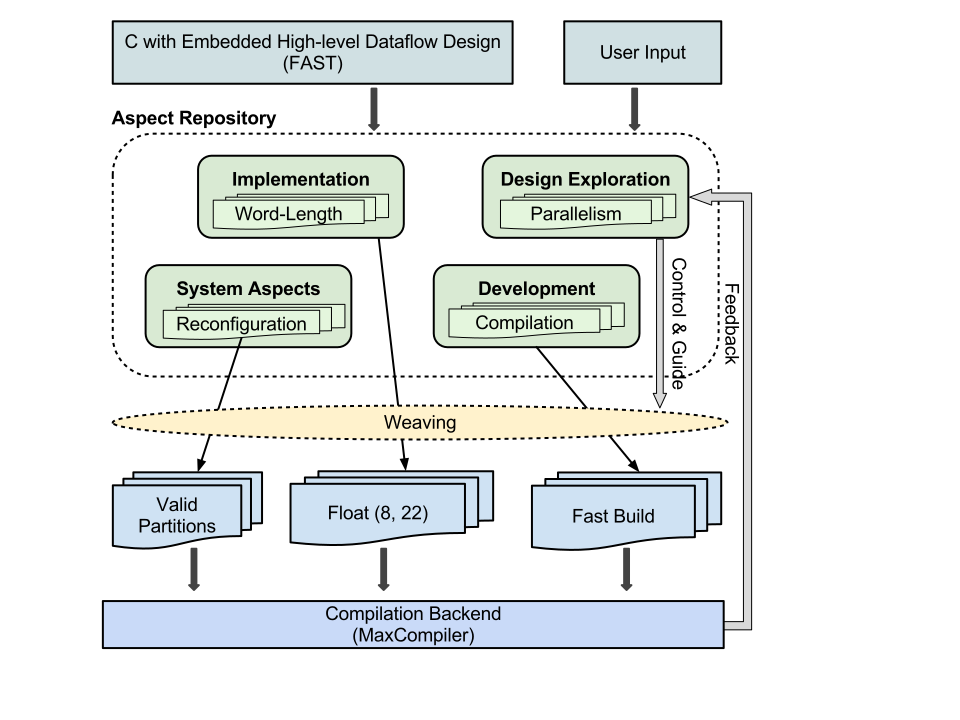
\includegraphics[scale=0.5, trim=60 50 0 0]{figs/asap13-design-flow.pdf_tex}
  \caption{Proposed approach for aspect-driven compilation of dataflow
    designs.}
  \label{fig:design-flow-overview}
\end{figure}

The design flow produces as its output a number of implementations based on
requirements specified through aspects.

The following algorithm describes the operation of the proposed design flow:

\begin{lstlisting}
  for (in as do als)
\end{lstlisting}
\end{comment}

\section{Design Goals}

Our design flow aims to improve both \emph{efficiency} (in terms of
performance and energy consumption) and \emph{productivity}. The
former is crucial to High Performance Computing, the latter helps
reduce development cost and time and is a well-known issue with
existing FPGA based acceleration solutions \XXX{cit. req.}. To achieve this we focus
on maintaining or improving the \emph{performance} and \emph{energy
  efficiency} of existing applications while using a more systematic
approach for design optimisation that results in more \emph{portable}
application code, improves \emph{integration} with existing
applications and \emph{automate} time consuming and error-prone tasks
that need to be performed manually using traditional tools.

\subsection{Performance and Energy Efficiency}
When targeting HPC applications it is crucial that our design flow
results in high-performance, highly efficient designs. To achieve this
we start by looking at some existing high-performance designs
(e.g. Reverse Time Migration -- see \Cref{sec:RTM}) and identify some
of the key requirements of these designs. Based on these observations
we require our approach to:

\begin{itemize}

\item \textbf{Computation is the most significant part} of
  high-performance applications. For stencil computations this is
  usually a fairly large stencil operation over a large number of
  adjacent data-points (multiple points in each dimension). For
  example, the RTM kernel uses two stencil operations of 31 floating
  point additions, 18 floating point multiplications and 1
  subtraction (\Cref{app:rtm-kernel}, Lines \ref{app:rtmk-op1} and
  \ref{app:rtmk-op2}).  Additionally, these are replicated a
  \texttt{Par} times (with Par as large as 12) which leads to a total
  of $((31 + 18 + 1) * 2 * 12) = 1200 $ floating point operations to
  be executed on each kernel cycle (in reality floating point
  operations are pipelined across 13 kernel cycles, but this is,
  generally, transparent to the user). Hence, our approach must
  provide a clear and concise manner to express computation
  (preferably standard operators).

\item Another crucial aspect in achieving high-performance is
  \textbf{replicating the design} across to chip to maximise speedup subject to
  maximum available bandwidth. This makes use of FPGA cache (around
  4MB of fast-local memory) to reuse data across time steps. This
  pipeline replication is achieved through design parametrisation and
  loops whose bounds are known at compile-time. The parameters that
  indicate the pipelining factor are shared across the compute and
  memory kernels but also across the CPU code.

\item High-performance designs \textbf{maximise usage of on-board
    DRAM}. Especially for stencil type computations where a number of
  time step iterations are performed over the original data, it is
  crucial to have the data available in the large, high bandwidth
  on-board DRAM rather than on the CPU side. Bandwidth of the on-board
  DRAM is 40GB/s compared to 2GB/s over PCI-Express to CPU. However,
  supporting DRAM introduces the additional complexity of managing
  multiple kernels (since memory read and write commands are,
  preferably, generated from kernels separated from the original
  dataflow kernel -- see \Cref{app:mem-read-kernel})
  and. Additionally, special API calls for generating the read/write
  commands have to be supported (\Cref{app:mem-read-kernel}, Line
  \ref{app:memrk-dram}).

\item \textbf{Expose optimisation opportunities for backend
  tools}. For example, our MaxCompiler backend supports some degree of
  trade-offs when mapping computation to DSPs. Additionally various
  trade-offs can be achieved by disabling pipeline depth etc.  These
  optimisations present interesting opportunities for trade-offs that
  enable developers to increase the number of parallel pipelines on
  the chip by balancing resource usage, or possibly reducing clock
  frequency.

\item Additionally, it has been recently showed that run-time
  reconfiguration can be used to improve the performance and
  energy-efficiency of FPGA designs. \XXX{Cit. req., more details} Our
  approach should therefore enable specification of designs with
  run-time reconfiguration both in the static flavour presented in
  \cite{Xinyu:Qiwei:Luk:Qiang:Pell:2012} where partitions are
  generated and scheduled optimally at compile-time but also in a
  dynamic, self-adaptive fashion \cite{6322875} in which the
  application can dynamically based on application inputs.

\end{itemize}

\XXX{Formulae for reducing clock frequency vs pipelining}

\XXX{Formulae for measuring energy efficiency/consumption with run-time reconfiguration}

\subsection{Productivity}

\subsubsection{Portability}

In the context of our design flow \emph{portability} refers to two
different aspects:
\begin{itemize}
\item \emph{portability of transformations and optimisations} -- it
  should be possible to reuse optimisation strategies in the context
  of different applications with as less user input as possible; in
  the context of RTM this is no longer possible: the transformation
  steps from the original naive implementation have been lost, and are
  now part of the existing code base. Of course these could be
  recovered, from version control for example, but a version control
  patch could obviously not be applied to other applications to
  generate highly pipelined designs. In other words if the developer
  was faced with the task of accelerating a similar computational
  kernel (which is likely since stencil computations follow a clear
  pattern) he would have to re-do all steps, resulting in a large
  decrease of productivity.

\item \emph{portability of designs over various FPGA devices} --
  generally resource available to FPGA chips vary greatly based on the
  chip manufacturer. Even in the simple case of chips produced by the
  same manufacturer, the reduction of a specific resource could
  prevent a design from working on a different FPGA chip. Hence
  designs cannot be considered portable, since a finely tuned design
  could not build on a different chip. By automating the design
  exploration process and identifying trade-offs automatically the
  optimisation process can be repeated for various devices without
  user input.
\end{itemize}

\XXX{Formulae for cost of automatic optimisation including design
  space exploration and compute cost vs cost of manual developer
  intervention}

\subsubsection{Integration}

It is important to facilitate the integration of application code
resulting from our approach with existing application code. For this
it should be possible to switch seamlessly between existing software
only code and. To achieve this we introduce a set of pragmas
(described in detail in \Cref{}) that allow users to switch between a
standard software compiler and the FAST compiler (\texttt{fastc}) to
automatically enable or disable hardware acceleration.

By using C99 syntax, FAST is able to share configuration parameters
with the CPU code (e.g. via constants or macro definitions),
simplifying management and integration of the CPU and dataflow kernel.

\XXX{More details...}

\subsubsection{Automation}

Automating the design space exploration process results in
productivity improvements. However we provide input points in our
design flow which can be used gradually to tweak and guide the
compilation process.

\XXX{More details...}

\section{Steps}

To meet these requirements we propose the following approach.


The proposed design flow is illustrated in Fig.~\ref{fig:design-flow}
and follows the steps:
\begin{enumerate}
\item a C application containing an embedded high-level dataflow
  design is developed from the original source application. The design
  is implemented using \FAST{} as described in Section~\ref{sec:maxc};
\item the dataflow design is transformed by the aspects in the
  repository to generate new designs (e.g. with multiple word-length
  configurations). The classes of aspects used with our approach are
  introduced in Section~\ref{sec:aspects};
\item the generated configurations are compiled using a backend
  compilation toolchain (currently MaxCompiler) to dataflow designs
  implemented on FPGAs;
\item the feedback from the compilation process is used to drive the
  design space exploration, repeating the weaving and compilation
  process until user specified requirements are met.
\end{enumerate}


\begin{figure}[!ht]
  \centering
  \def\svgwidth{\textwidth}
  \input{figs/asap13-design-flow.pdf_tex}
  \caption{Proposed approach for aspect-driven compilation of dataflow
   designs.}
  \label{fig:reconfig-design-flow}
\end{figure}

Compared to existing work described in
\cite{Cardoso:Teixeira:Alves:Nobre:Diniz:Cutinho:Luk:2012} and
\cite{cardoso2011new} our approach emphasises and provides more
freedom in the exploration of design level optimisation (such as word
length optimisations and mapping of arithmetic blocks to DSPs) by
using a combination of implementation aspects (shown in
Fig.~\ref{fig:design-flow}) and \FAST{} optimisation options.

Additionally, our approach targets a dataflow architecture as opposed
to the von Neumann architecture proposed in related work, which
typically includes a General-Purpose Processor (GPP) and a custom
accelerator. We consider additional optimisations to achieve
performance improvements as a result of a systematic design space
exploration process.

\section{Components}

Firstly, we introduce \FAST{} (described in Section \ref{sec:maxc}), a
novel language for specifying dataflow designs. We specify the
accelerated portion of the original applications using \FAST{}
dataflow kernels. By maintaining compatibility with C99 syntax we
improve developer productivity by providing a familiar language and
introduce the possibility of combining hardware and software
specifications. Secondly, by using an aspect driven compilation flow
we decouple optimisation from design development, improving design
portability, and we automate the generation of code and design space
exploration improving productivity. Finally, systematic design space
exploration is used to identify maximum performance configurations,
subject to platform specific constraints.

\subsection{FAST Dataflow Designs}

Dataflow designs are to be described in FAST, a novel dataflow
language. FAST uses simple C99 style syntax to capture the computation
data path and control-path and acts as a layer on top of the
MaxJ/MaxCompiler designs in our approach.

\subsection{LARA Aspect Descriptions and Harmonic Aspect Weaver}

We use LARA and the Harmonic aspect weaver to implement the aspect
descriptions that drive the compilation process.

\subsection{MaxCompiler Backend}

The target of our compilation is a fully functional MaxCompiler design.
This involves automatic generation of:
\begin{itemize}
\item compute kernels
\item memory access kernels
\item managers
\item run-time API calls to be inserted in the original application code
\end{itemize}


\section{Comparison with Existing Approaches}

\XXX{Compare with MaxCompiler}

\XXX{Compare with Vivado or other similar tools}

\section{Extensions}

We present our extensions to the original design flow required to
support run-time reconfiguration.

\subsection{Design Modelling}

A design model for resource usage, pipeline depth and timing
information can created using limited user input. This is to be used
in the run-time reconfiguration to determine optimal partition
scheduling.

\begin{figure}[!ht]
  \centering
  \def\svgwidth{\textwidth}
  \input{figs/rep-modelling.pdf_tex}
  \caption{High-level aspects controlling generation of design
    resource, performance and timing modelling.}
  \label{fig:reconfig-design-flow}
\end{figure}

Based on this model we can estimate design performance, latency,
energy efficiency and compilation time, and provide useful feedback
earlier in the development process than is possible with existing
tools.

Of course our model relies on user inputs for resource usage map
relies on estimates for resource usage and will not be expected to
provide very accurate results, especially in the presence of
optimisation of backend tools and various trade-offs that can be made
when mapping arithmetic to FF/LUT pairs vs DSPs.

\subsection{Run-time Reconfiguration Support}

Extensions to the original flow are required to support the automation
of run-time reconfiguration support. Figure
\ref{fig:reconfig-design-flow} presents an overview of the revised
design flow.

\begin{figure}[!ht]
  \centering
  \def\svgwidth{\textwidth}
  \input{figs/fpt13-design-flow.pdf_tex}
  \caption{Revised design flow to support run-time reconfiguration}
  \label{fig:reconfig-design-flow}
\end{figure}

\begin{enumerate}
\item From an initial C + FAST design we create a number of
  configurations by applying implementation and system aspects as
  described in ASAP.
\item For each configuration we derive a model of the resource usage,
  performance and power usage using modelling aspects (described in
  section 3)
\item Based on predicted models (from step 2) and possibly on existing
  empirical information from the Design DB we partition the
  application and schedule the partitions to achieve user requirements
  and optimization goals.
\item Finally a number of executables and designs are created,
  corresponding to the generated configurations from step 3. Based on
  compilation and execution (of automated performance tests) we refine
  our predictions for design resource usage, performance and power.
\end{enumerate}

Additionally the run-time environment has to be extended to support
this approach. An overview of the assumed runtime architecture for the
proposed approach is shown in Figure \ref{fig:reconfig-runtime}.

\begin{figure}[!ht]
  \centering
  \def\svgwidth{\textwidth}
  \input{figs/fpt13-runtime.pdf_tex}
  \caption{Run-time architecture required to support run-time reconfiguration}
  \label{fig:reconfig-runtime}
\end{figure}

\begin{enumerate}
\item The CPU drives the FPGA. It initiates the computation and
  monitors the FPGA for factors such as temperature and power.
\item The CPU can request the FPGA to abort execution of the current
  design. Current results are saved (i.e. streamed back to CPU)
  before reconfiguration is triggered.
\item The CPU can select a new design to be uploaded and
\item Empirical results are recorded in the Design Database, to
  improve future estimates of performance, power and thermal values.
\end{enumerate}

\section{Summary}

\section{The  MaxC Language}

MaxC is a novel language for specifying dataflow designs. It is based
on the widely used C99 standard which makes it familiar and easy to
adopt for developers facilitating translation of existing application
code to dataflow designs. The simple syntax of C99 facilitates
integration with other tools (such as aspect weavers), allowing the
language to interact well with existing compilers or source to source
translation frameworks (e.g. LARA, ROSE), allowing source level
optimizations to be applied through different tools. MaxC itself is a
simple language, which is intended to be used for expressing the
simplest form of a dataflow design. Optimizations and other
transformations are encapsulated in aspects which are developed
separately and applied through aspect weaving. This results in a more
flexible approach for generating and exploring the space of efficient
dataflow designs.

\begin{comment}
  We identify the following requirements for any dataflow language:
  \begin{enumerate}
  \item intuitive and easy to use
  \item facilitate translation of existing applications
  \item interacts well with
    high-level tools
  \end{enumerate}
\end{comment}

Since MaxC is compiled to MaxJ it uses the same execution model: a
design is composed of one or more computational kernels (which
implement the functionality we are interested in) which are connected
to form a design. Communication between kernels is asynchronous, so
kernels can operate independently of each other but computation within
kernels is synchronous, so a kernel will compute only when all it's
active inputs have values available.

Figure \ref{fig:maxc-1dconv} shows an example MaxC dataflow kernel
which implements a 1D convolution computation used to value European
options.


\lstset{style=MaxC}

\begin{figure}
  \begin{lstlisting}
    void kernel_Convolution1D(float* p, float c_0_0_0, float c_p_0_0, float c_n_0_0, int n1, int ORDER, float* out)
    {

      in(p);

      float* i4 = count(1000, 1);
      float* i1 = countChain(n1, 1, i4);

      #pragma maxc DSPBalance:full
      int result =
        p[0]  * c_0_0_0 +
        p[1]  * c_p_0_0 +
        p[-1] * c_n_0_0;

      int up =(i1 >= ORDER) && (i1 < n1 - ORDER);

      out = up ? result : p;

      out(out);
    }
  \end{lstlisting}
  \caption{Example MaxC design for a 1D convolution kernel.}
  \label{fig:maxc-1dconv}
\end{figure}

\subsection{Kernels}

Kernels are defined as regular C functions, with the ``kernel\_''
identifier prepended (Line 1). The inputs and outputs of the kernel
are clearly specified in the header, inputs followed by outputs. At
the kernel level MaxC captures the dataflow elements by using:

\begin{itemize}
\item \emph{regular C constructs} are used as much as possible to make
  the language more intuitive. This includes standard C99 types and
  conventions for implementing kernels. Some overloaded operators are
  provided such as the array access operators to provide a more
  succinct syntax for accessing ``past'' or ``future'' stream elements
  (Lines 15 -- 17).

\item \emph{pragma directives} are used to convey additional
  information to the compiler for which C99 does not provide flexible
  built-in constructs (e.g. specifying type width) or additional
  optimization hints (e.g. the DSP balance, Line 13);

\item \emph{specific API calls} are used for higher level constructs
  such as inputs and outputs (Lines 8, 24), counters (Lines 10 -- 11).

\end{itemize}


Figure \ref{fig:maxc-1dconv} shows the main elements of a MaxC design:

\begin{enumerate}
\item \emph{inputs and outputs} are declared in the kernel header and
  connected in the kernel body. Lines 2-6 show the kernel declaration
  specifying the stream input "p" and output "out" as well as a number
  of scalar parameters configurable at run-time. API calls are used to
  connect these inputs (Line 7 and 22);

\item \emph{control} elements are implemented either via standard C99
  constructs (such as conditional statements or operators) or via API
  calls that enable multiplexing between 2 or more streams;

\item \emph{computation} is implemented using regular C99 syntax and
  semantics. The MaxCC backend will also automatically translate
  standard functions in the C99 math library to hardware blocks for
  common functions such as square root, exponential, logarithms.

\item \emph{streams} are represented as regular C99 pointers. For
  example Line 2 declares a stream of float values names ``p''.
  Normal array notation can be used to generate either previous
  (negative indices) or future values (positive indices) or
  dereference the stream to get the current stream value. Negative
  indices are allowed (as on Line 16). On lines 13-16 we use array
  index notation to access future (positive offset) or past (negative
  offset) stream elements. Supported offset expressions are linear
  expressions comprised of constants or variables (either loop
  induction variables, or normal variables but for which a compile
  time range of values is specified -- this is required to generate
  efficient hardware).

\item \emph{compile time constructs} such as loops are supported as
  long as their bounds are known at compile time.

\item \emph{optimizations} can be applied via pragmas (Line 12) or API
  calls. Additional type information can also be provided via pragmas.

\end{enumerate}

The MaxC API provides a number of useful, higher-level constructs.
such as output functions that are used to connect an internal kernel
stream to the output stream of a kernel, various counters and counter
chain configurations that can be instantiated using functions from the
counter API (Lines 9 -- 10) or functions such as stream\_select that
are used to multiplex between a number of streams based on the value
of condition stream.


\begin{comment}
\subsection{Designs}

MaxC also allows specification of designs using multiple kernels. This
involves selecting the kernel instances and connecting them as well as
setting a number of design configuration and compilation options such
as operating frequency.

Figure \ref{lst:maxc-design} illustrates the design for the 1D
convolution example which places and connects memory command kernels
to control the generation of memory streams and the actual computation
kernels.

On Lines 3-6 we specify the kernel instances. On Lines 8 -- 10 we
connect these. Lines 13 -- 15 specify the design frequency, the memory
clock frequency and enable the addition of debug elements.

\begin{figure}[!h]
  \centering
  \begin{lstlisting}
    void design_Convolution1D() {
      // kernels
      kernel_t k1 = kernel_init(kernel_Convolution1D);
      kernel_t k2 = kernel_init(kernel_Cmdwrite);
      kernel_t k3 = kernel_init(kernel_Cmdread);

      // connections
      connect2(k1, k2);
      connect3(k1, k2, ``a'');
      connect4(k1, k3, ``a'', ``b'');

      // configuration
      set_frequency(150);
      set_memory_frequency(333);
      set_enable_debug(true);
    }
  \end{lstlisting}
  \caption{MaxC design specification, connecting multiple kernels and
    setting various configuration options}
  \label{lst:maxc-design}
\end{figure}
\end{comment}

\section{Aspect Descriptions}
\begin{frame}
  \frametitle{3. Aspect Descriptions}
  \begin{enumerate}
    \setlength{\itemsep}{15pt}
  \item \textbf{System Aspect Descriptions}
    \begin{itemize}
    \item FAST + C application
    \end{itemize}
  \item \textbf{Implementation Aspect Descriptions}
    \begin{itemize}
    \item FPGA and dataflow specific optimisations
    \end{itemize}
  \item \textbf{Exploration Aspect Descriptions}
    \begin{itemize}
    \item user guided design space exploration strategies
    \end{itemize}
  \item \textbf{Development Aspect Descriptions}
    \begin{itemize}
    \item automate repetitive, error-prone development tasks
    \end{itemize}
  \end{enumerate}
\end{frame}

\begin{frame}{System Aspects: Run-time Reconfiguration}
  \begin{itemize}
  \item idle functions may appear in large designs
  \item use run-time reconfiguration to remove idle functions
    \begin{columns}
      \begin{column}{.55\textwidth}
  \begin{figure}[!ht]
    \centering
    \def\svgwidth{\linewidth}
    \input{figs/rtm-desc.pdf_tex}
  \end{figure}
      \end{column}
      \begin{column}{.45\textwidth}
  \begin{figure}[!ht]
    \centering
    \def\svgwidth{\linewidth}
    \input{figs/rtm-idle.pdf_tex}
  \end{figure}
      \end{column}
    \end{columns}


  \end{itemize}
\end{frame}

\begin{frame}[fragile]{System Aspects: Run-time Reconfiguration}
  \begin{itemize}
    \setlength{\itemsep}{8pt}
  \item pragmas specify configuration parameters
\end{itemize}
    \begin{columns}
      \begin{column}{.7\textwidth}
        \begin{center}
          \begin{lstlisting}[style=MaxC]
#pragma fast hw:f1 cfg:c0(Par=2)
x = f(0);
#pragma fast hw:f1 cfg:c1(Par=1)
y = f(x);
#pragma fast hw:g1 cfg:c1(Par=1)
z = g(x, y);
          \end{lstlisting}
        \end{center}
      \end{column}
      \begin{column}{.3\textwidth}
        {\footnotesize
          \begin{table}[!h]
            \renewcommand{\arraystretch}{1.3}
            \hspace{-2cm}
            \begin{tabular}{c|c|c}
              \multicolumn{3}{c}{\bf{partition}} \\
              \hline
              \bf{call.key} & \bf{hw} & \bf{cfg}  \\
              \hline
              main:f:1 & fast\_f0 & c0 \\
              main:f:2 & fast\_f1 & c1 \\
              main:g:3 & fast\_g & c1 \\
            \end{tabular}
          \end{table}
        }
      \end{column}
    \end{columns}

\end{frame}

\begin{frame}[fragile]{3. Aspect Descriptions}
  \frametitle{ System Aspects: Run-time Reconfiguration}
  Map function calls (on the CPU side) to configurations:
  \begin{itemize}
  \item inspect each function call
  \item if part of a partition, add corresponding FAST pragma
  \item $ \text{partition} : \text{funcCall} \rightarrow (\text{kernel}, \text{config}) $
  \end{itemize}

  \begin{lstlisting}[style=lara]
aspectdef AspReconfig
  input: partition
  function.call:
    if (call.key in partition) {
     p = partition[call.key]
     config = p.cfg + '(Par = ' + p.par + ')'
     kernel = p.par
     call.prepend('#pragma fast hw:'kernel' cfg:'config)
    }
end
  \end{lstlisting}
\end{frame}


\begin{frame}[fragile]{3. Aspect Descriptions}
  \frametitle{Implementation Aspects: Operator Optimisation}
  Map computation to Digital Signal Processors:
  \begin{itemize}
  \item $ \text{opMapping} : \overrightarrow{\text{opOccurence}} \rightarrow \text{factor}$
  \item $\text{factor} \in \{\text{none}, \text{balanced}, \text{full}\} $
  \item mapping can be varied by different aspect to support design
    space exploration
  \end{itemize}
  \begin{lstlisting}[label=lst:label, style=lara]
aspectdef DspBalancing
input: opMapping
 function.stmt:
   opUsage = countOperatorUsage(stmt)
   factor  = opMapping[opUsage]
   if (factor != '')
     stmt.prepend('#pragma fast balanceDSP:' + factor);
end
  \end{lstlisting}
\end{frame}

\begin{frame}{3. Implementation Aspects: Operator Optimisation}
  \begin{figure}[!ht]
    \centering
    \def\svgwidth{\linewidth}
    \input{figs/opt-split.pdf_tex}
  \end{figure}

\end{frame}

\begin{frame}[fragile]{3. Aspect Descriptions}
  \frametitle{Exploration Aspect Descriptions: Iterative Exploration}
  Automate design space exploration
  \begin{itemize}
  \item vary an attribute of a dataflow configuration
  \item generate FAST configuration and compile FPGA bitstream
  \item extract feedback from compilation report
  \item stop when a resource usage limit is reached
  \end{itemize}
  \begin{lstlisting}[label=lst:label, style=lara]
aspectdef DesignExploration
input: attribute, start, step, res, res_limit, config
  config[attribute] = start
  do {
    var designName = genName(config)
    generateFASTDesign(designName, config)
    buildFASTDesign(designName)
    config[attribute] += step
  } while (@hw[designName].res < res_limit)
end
  \end{lstlisting}
\end{frame}

\begin{frame}[fragile]{Monitoring and Logging}
  \begin{itemize}
  \item Logging: useful for debugging (no run-time support)
  \end{itemize}
  \begin{lstlisting}[label=lst:label, style=lara]
aspectdef WatchVar
function.vref{is_written}:
  vref.parent.prepend('log("vref.name", vref.name)')
  vref.parent.append('log("vref.name", vref.name)')
end
  \end{lstlisting}

  \begin{itemize}
  \item Monitoring: useful for profiling
  \end{itemize}
  \begin{lstlisting}[label=lst:label, style=lara]
aspectdef LoopMonitor
function.loop{is_innermost}:
  entry:   prepend(mon_iterationIn())
  exit :   append (mon_iterationOut())
  default: prepend(mon_instanceIn())
           append(mon_instanceOut())
end
  \end{lstlisting}
\end{frame}

\begin{frame}{\texttt{fastc}}
  \begin{figure}[!ht]
    \centering
    \def\svgwidth{\linewidth}
    \input{figs/comp-flow.pdf_tex}
  \end{figure}
  \begin{itemize}
    \setlength{\itemsep}{10pt}
  \item experimental compiler for FAST
  \item supports all dataflow features
  \item portability: aspects, high level pragmas
  \item optimisations: low-level pragmas, inference
  \end{itemize}
\end{frame}

\section{Evaluation}

\subsection{RTM Implementation}
We evaluate the proposed approach by implementing a high-performance
application based on the Reverse Time Migration method for seismic
imaging which is used to detect geological structures, based on the
Earth's response to injected acoustic waves. The technique models the
propagation of injected waves using the isotropic acoustic wave
equation \cite{araya2011assessing}:
\begin{align}
\frac{d^2p(r,t)}{dt^2} + {dvv(r)}^2\bigtriangledown^2p(r,t) = f(r,t)
\end{align}
We approximate the differential equation using stencil computation to
perform a fifth-order Taylor expansion in space and first-order Taylor
expansion in time.

We use \MAXC{} to implement the dataflow kernels and aspects to generate
multiple configurations for the design by creating two kernels that
are used to control the memory command read and write streams
(CmdRead, CmdWrite) and the computation kernel (RTM).  To illustrate
the potential benefits of our approach we analyse the results of using
the debugging aspect of Section \ref{sect:asp_debug}. Table
\ref{table:loc} compares the number of lines of code required for the
original \MAXC{} + Aspect implementation with the equivalent MaxCompiler
implementation showing a reduction in code size of up to 42\% for the
run-time reconfigurable design and a reduction in the number of API
calls (including debug calls) of up to 67\% which translate to
increased productivity.

\begin{table}[!h]
  \renewcommand{\arraystretch}{1.3}
  \centering
  \caption{Code measures for the RTM kernels comparing \MAXC{} and
    MaxCompiler.}
  \label{table:loc}
  \begin{tabular}{c|ccc|cc}
    \hline
    \multirow{2}{*}{\bf{Kernel}} & \bf{Aspect } & \multicolumn{2}{c|}{\bf{\MAXC{}}} & \multicolumn{2}{c}{\bf{MaxCompiler}}                   \\
    \                            & \bf{LOC}     & \bf{LOC}                       & \bf{\# API calls} & \bf{LOC} & \bf{\#API Calls} \\
    \hline \hline
    CmdRead                      & 12           & 26                             &      6         & 59       &      39        \\
    CmdWrite                     & 12           & 28                             &      39        & 79      &       56         \\
    RTM Static                   & 12           & 246                            &     43         & 403     &       175        \\
    RTM RTR                      & 12           & 377                            &     91         & 669     &       275       \\
  \end{tabular}
  \vspace{-3mm}
\end{table}

\subsection{Results}

Results of the design space exploration using the aspect in
Fig.~\ref{fig:aspect-exploration} with variable mantissa illustrate
the trade-offs between accuracy and resource usage
(Fig.~\ref{fig:precision}). We observe irregular, large variations
when decreasing the mantissa from 18 to 16 and 24 to 22 which is the
effect of the backend tools mapping arithmetic to a combination of
both DSPs and LUT/FF elements. The mantissa boundaries at which this
optimisation occurs are platform specific, depending on the
architecture of the DSPs. Hence automating this optimisation via
aspects and decoupling it from the original source code makes the
application more portable and facilitates discovery of interesting
trade-off opportunities using design space exploration.

\begin{figure}[!h]
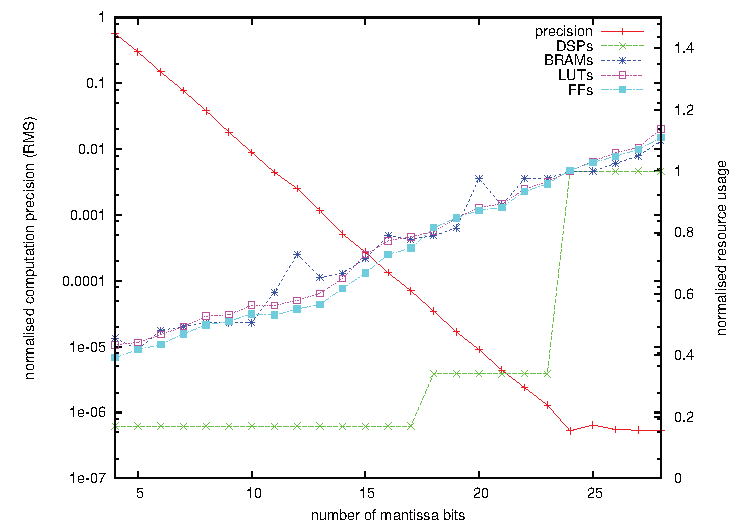
\includegraphics[scale=0.7]{figs/pre}
\caption{Exploration of accuracy vs resource usage trade-offs using the aspect
shown in Fig.~\ref{fig:aspect-exploration} with variable mantissa.}
\label{fig:precision}
  \vspace{-2mm}
\end{figure}

The DSP balancing aspect shown in Fig.~\ref{fig:aspect-DSP} allows to
explore the resource trade-offs of implementing arithmetic operations
in either DSPs or LUTs and FFs (Fig.~\ref{fig:arith}) and helps to
avoid over mapping on DSPs for arithmetic intensive applications.

\begin{figure}[!h]
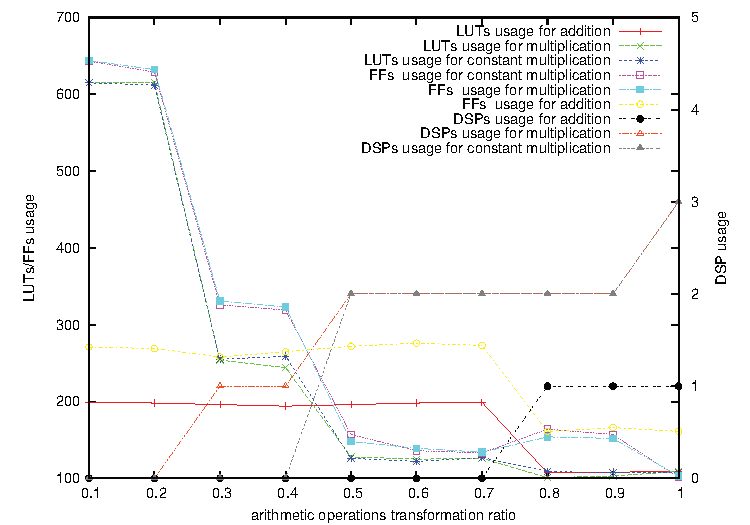
\includegraphics[scale=0.7]{figs/arith}
\caption{Exploration of DSP and LUT/FF balancing for functional units
  implementing a single arithmetic operation using the aspect shown
  in Fig.~\ref{fig:aspect-DSP}.}
\label{fig:arith}
  \vspace{-2mm}
\end{figure}

Design space exploration using the aspect in
Fig.~\ref{fig:aspect-exploration} with increasing parallelism level
can be used to investigate design scalability. For example for the
described RTM implementation, Fig.~\ref{fig:scalability} shows that
performance scales linearly with the number of parallel pipelines and
that significant speedups can be obtained by the \MAXC{} dataflow
design compared to the CPU only implementation. Depending on the
problem size, our approach can be used to achieve a significant
speedup over software only versions which is comparable with the best
published FPGA results for static designs
\cite{Xinyu:Qiwei:Luk:Qiang:Pell:2012}, \cite{araya2011assessing}.

\pgfplotsset{every axis x label/.style={
  at={(0.5,0)},
  below,
  yshift=-5pt}}

\pgfplotsset{every axis y label/.style={
  at={(0,0.5)},
  xshift=-20pt,
  rotate=90}}

\begin{figure}[!h]
  \centering
  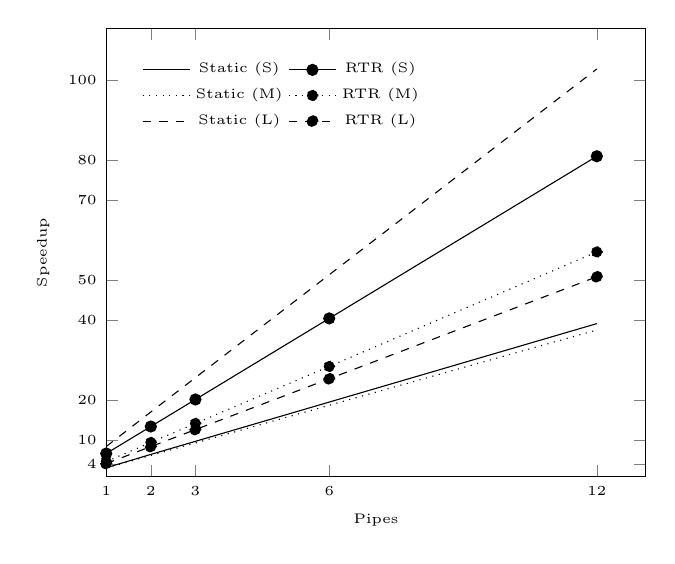
\begin{tikzpicture}
    \selectcolormodel{gray}
    \begin{axis}[
        xmin=1,
        ymin=1,
        %no markers,
        font=\tiny,
        xlabel=Pipes,
        ylabel=Speedup,
        xtick={1,2,3,6,12},
        ytick={4, 10, 20, 40, 50, 70, 80, 100},
        legend columns=2,
        legend entries={
          Static (S),
          RTR (S),
          Static (M),
          RTR (M),
          Static (L),
          RTR (L)},
        legend style={
          draw=none,
          at={(0.05,0.85) },
          anchor=west
        }
      ]

      \addplot[mark=none] coordinates {
        (1, 3.2)
        (2, 6.53)
        (3, 9.8)
        (6, 19.6)
        (12, 39.2)
      };
      \addplot[mark=*] coordinates {
        (1, 6.75)
        (2, 13.5)
        (3, 20.25)
        (6, 40.5)
        (12, 81)
      };
      \addplot[dotted] coordinates {
        (1, 3.13)
        (2, 6.26)
        (3, 9.4)
        (6, 18.8)
        (12, 37.6)
      };
      \addplot[mark=*, dotted] coordinates {
        (1, 4.75)
        (2, 9.51)
        (3, 14.27)
        (6, 28.5)
        (12, 57.1)
      };
      \addplot[mark=none, dashed] coordinates {
        (1, 8.5)
        (2, 17.13)
        (3, 25.7)
        (6, 51.4)
        (12, 102.8)
      };
      \addplot[mark=*, dashed] coordinates {
        (1, 4.25)
        (2, 8.48)
        (3, 12.725)
        (6, 25.42)
        (12, 50.9)
      };2
    \end{axis}
  \end{tikzpicture}
  \caption{Scalability of the RTM dataflow design explored using the aspect
shown in Fig.~\ref{fig:aspect-exploration}.}
  \label{fig:scalability}
  \vspace{-2mm}
\end{figure}

Fig.~\ref{fig:scalability} also shows a model of the performance
benefits of using a run-time reconfiguration implementation which is
generated by using the reconfiguration aspect of Fig. 4 to create two
configurations for the RTM \MAXC{} kernel. Since, in our model, during
the first half of the execution time, the backward propagation and
imaging functions are idle, the first configuration requires only half
the resources. Hence, the number of parallel pipelines can be doubled,
halving the execution time of the first configuration. The speedup
obtained is comparable to \cite{Xinyu:Qiwei:Luk:Qiang:Pell:2012}, but
the partitioning and optimisation exploration process is automated via
aspects, which increases developer productivity. The automated process
improves portability of the design, allowing optimisations based on
design space exploration to be carried out on various platforms (hence
subject to varying resource constraints) without manual intervention.

\section{Related Work}

A number of dataflow languages have been developed targeting FPGAs but
also multi-core platforms. Table \ref{table:feature-comparison}
summarises some of the important features of these languages compared
to \MAXC{}.

Lucid \cite{ashcroft1977lucid}, SISAL \cite{gurd1987implicit},
\cite{mcgraw1983sisal} and Lustre \cite{halbwachs1991synchronous}, are
examples of functional dataflow languages. The latter is based on a
synchronous programming model, facilitating safety verification for
critical software \cite{halbwachs1992programming} rather than
performance. The functional programming style complicates the
translation of existing imperative applications and none have existing
implementations for FPGAs, so a performance comparison is not
possible.

Streams-C\cite{Gokhale:Stone:Arnold:Kalinowski:2000} and
ImpulseC\cite{ImpulseC} adopt imperative ANSI C syntax and an
execution model based on Communicating Sequential Processes and
introduce non-standard syntax and constructs for specifying designs
such as special comment blocks which are used to annotate the C
application code. The specialised syntax makes the languages harder to
integrate with existing source-to-source translation or aspect weaving
frameworks.

Hybrid approaches such as MaxCompiler\cite{5719584} separate the CPU
run-time component from the accelerated one, providing a C run-time
environment and a Java API for building dataflow designs via
meta-programming. The separation complicates the development process,
hindering sharing of design parameters and, consequently, the design
space exploration process. The use of meta-programming simplifies
design parametrisation, but can make resulting programs harder to
understand. In contrast, the proposed approach allows the computation
description, which includes CPU and dataflow components, to be specified
using a single language and to be decoupled from design
parametrisation and other optimisation strategies which are captured
as LARA aspects. This separation of concerns results in more intuitive
and maintainable descriptions.

\begin{table*}[!ht]
  \renewcommand{\arraystretch}{1.8}
  \centering
  \caption{Feature comparison of the \MAXC{}/LARA approach and existing dataflow implementations.}
  \label{table:feature-comparison}
  \begin{tabular}{ p{1.7cm} |  p{1.8cm} |  p{1.8cm} |  c | c | l | l}
    \hline
    \bf{Language}          & \bf{Syntax}          & \bf{Paradigm}               & \bf{Support}              & \bf{Implementation}   & \bf{Design Parametrisation}            & \bf{Optimisation Strategies}          \\
    \hline \hline
    \bf{Lucid}                    & Lucid                & Functional                  & \multirow{3}{*}{Software}                  & \multirow{3}{*}{Multiprocessor}        & \multirow{3}{*}{\begin{minipage}{0.7in}Manual Source Transformation\end{minipage}} & \multirow{5}{*}{Manual Code Revision} \\
    \bf{SISAL}                    & SISAL                & Functional                  &                &    &                                        &                                       \\
    \bf{Lustre}                   & Lustre               & Synchronous                 &               &        &                                        &                                       \\
    \cline{1-6}
    \multirow{2}{*}{\bf{MaxCompiler}}              &  \multirow{2}{*}{\begin{minipage}{0.5in}C99(SW) Java(HW)\end{minipage}} &  \multirow{2}{*}{\begin{minipage}{1in}Imperative(SW) Dataflow(HW)\end{minipage}}      & \multirow{5}{*}{Combined}                  & \multirow{5}{*}{CPU + FPGA}                  & \multirow{2}{*}{Meta-programming}                      &                                       \\
    \cline{1-3}\cline{6}
    \multirow{2}{*}{\begin{minipage}{0.6in}\bf{Streams-C} \bf{ImpulseC}\end{minipage}}                & \multirow{2}{*}{C99}                  &      \multirow{2}{*}{\begin{minipage}{1in}Imperative(SW) CSP(HW)\end{minipage}}              &                   &                & \multirow{2}{*}{Compiler Directives}   &                                       \\
     \cline{1-3}\cline{6-7}
    \multirow{2}{*}{\bf{\MAXC{}}/\bf{LARA}} & \multirow{2}{*}{\begin{minipage}{1in}C99(SW) LARA(Aspects)\end{minipage}} & \multirow{2}{*}{\begin{minipage}{1in}Imperative(SW) Dataflow(HW) AOP(Aspects)\end{minipage}} &  & & \multicolumn{2}{c}{\multirow{2}{*}{\begin{minipage}{2.3in}Compiler Directives + \\ Automated Aspect-Directed Source Transformation\end{minipage}}}
                                                                                                                                \\
  \end{tabular}
\end{table*}

The use of LARA aspects in guiding the compilation process of C
applications is described in
\cite{Cardoso:Teixeira:Alves:Nobre:Diniz:Cutinho:Luk:2012} and
\cite{cardoso2011new} but the backend compilation targets a von
Neumann architecture (GPP + custom accelerator units) unlike the
dataflow architecture proposed in this paper. The approach described
in \cite{Cardoso:Teixeira:Alves:Nobre:Diniz:Cutinho:Luk:2012} and
\cite{cardoso2011new} relies more on high-level source transformation
whereas our approach is based on a systematic design space exploration
process, which enables the analysis of more low-level
optimisations. Finally,
\cite{Cardoso:Teixeira:Alves:Nobre:Diniz:Cutinho:Luk:2012} and
\cite{cardoso2011new} do not consider development aspects which can be
used to improve developer productivity.

The use of aspect-oriented programming for specifying strategies for
run-time adaptation of FPGA designs discussed in \cite{6322875}
differs from the static process considered in this paper in which the
application is partitioned and scheduled at compile time, to achieve
optimised performance as described in
\cite{Xinyu:Qiwei:Luk:Qiang:Pell:2012}. An advantage of our approach
is that an optimised allocation is generated prior to application
execution. However, we lack the flexibility of adapting the design to
varying input conditions.

\chapter{Conclusion}

\section{Results}

\section{Limitations}

\section{Future Work}

\emph{Extending the approach to other classes of parallel
  computation}.  Based on the evaluation results, I will investigate
extending the approach to support the generation of aspect
descriptions for additional classes of parallel computation such as
Sparse or Dense Linear Algebra, MapReduce or N-Body Simulation which
are quintessential examples of parallel kernels
\cite{Asanovic:Bodik:Catanzaro:Gebis:Husbands:Keutzer:Patterson:Plishker:Shalf:Williams:Yelick:2006}. This
step could also provide valuable feedback which can be used to refine
and validate the proposed approach.

\emph{Support MaxCompiler 2013.1}. MaxCompiler 2013.1 introduces a new
interface and interesting opportunities for optimisations. It
introduces the possibility to control groups of DFEs and...
\XXX{More details here}

\emph{Support a standardise set of pragams} such as OpenACC.

\emph{Extension to heterogeneous systems}. Apart from including
specific support for reconfiguration our approach is intentionally
platform agnostic to allow extension to other platforms for dataflow
computing (such as CPU and GPGPUs).

\emph{Extension to applications in other areas of finance}


% Note that IEEE typically puts floats only at the top, even when this
% results in a large percentage of a column being occupied by floats.


% An example of a double column floating figure using two subfigures.
% (The subfig.sty package must be loaded for this to work.)
% The subfigure \label commands are set within each subfloat command, the
% \label for the overall figure must come after \caption.
% \hfil must be used as a separator to get equal spacing.
% The subfigure.sty package works much the same way, except \subfigure is
% used instead of \subfloat.
%

% Note that often IEEE papers with subfigures do not employ subfigure
% captions (using the optional argument to \subfloat), but instead will
% reference/describe all of them (a), (b), etc., within the main caption.


% An example of a floating table. Note that, for IEEE style tables, the
% \caption command should come BEFORE the table. Table text will default to
% \footnotesize as IEEE normally uses this smaller font for tables.
% The \label must come after \caption as always.
%
%\begin{table}[!t]
%% increase table row spacing, adjust to taste
%\renewcommand{\arraystretch}{1.3}
% if using array.sty, it might be a good idea to tweak the value of
% \extrarowheight as needed to properly center the text within the cells
%\caption{An Example of a Table}
%\label{table_example}
%\centering
%% Some packages, such as MDW tools, offer better commands for making tables
%% than the plain LaTeX2e tabular which is used here.
%\begin{tabular}{|c||c|}
%\hline
%One & Two\\
%\hline
%Three & Four\\
%\hline
%\end{tabular}
%\end{table}


% Note that IEEE does not put floats in the very first column - or typically
% anywhere on the first page for that matter. Also, in-text middle ("here")
% positioning is not used. Most IEEE journals/conferences use top floats
% exclusively. Note that, LaTeX2e, unlike IEEE journals/conferences, places
% footnotes above bottom floats. This can be corrected via the \fnbelowfloat
% command of the stfloats package.


\section*{Acknowledgments}

The authors would like to thank Jacob Bower and Oliver Pell from
Maxeler Technologies Ltd. for their valuable comments on the paper and
constructive suggestions regarding our approach.

This work is supported in part by the China Scholarship Council, by
the European Union Seventh Framework Programme under grant agreement
number 257906, 287804 and 318521, by UK EPSRC, by Maxeler University
Programme, and by Xilinx.

% trigger a \newpage just before the given reference
% number - used to balance the columns on the last page
% adjust value as needed - may need to be readjusted if
% the document is modified later
%\IEEEtriggeratref{0}
% The "triggered" command can be changed if desired:
%\IEEEtriggercmd{\enlargethispage{-5in}}

\def\IEEEbibitemsep{3pt plus .5pt}
\bibliographystyle{IEEEtran}
\bibliography{../../refdb/bibliography.bib}



\end{document}
